\chapter{Principles}

This chapter describes basic informations about radiation environment, failure modes in electronic devices and introduction to RadFET dosimetry.

\section{Radiation on Low Earth Orbit}
    Radiation on LEO comes from trapped particle belts, solar particle events and cosmic rays \cite{ESA_radiation}. There are also other sources of radiation, but they are negligible comparing to those effects.

    \bigskip \textbf{Trapped particles}

    Electrons and protons are trapped in Earth's magnetic field, following magnetic field lines. They are a serious concern on Low Earth Orbit along polar regions and inside the South Atlantic Anomaly. In figure the \ref{Polar_SAA} radiation pattern along Earth is shown.

    \begin{figure}[H]
        \centering
        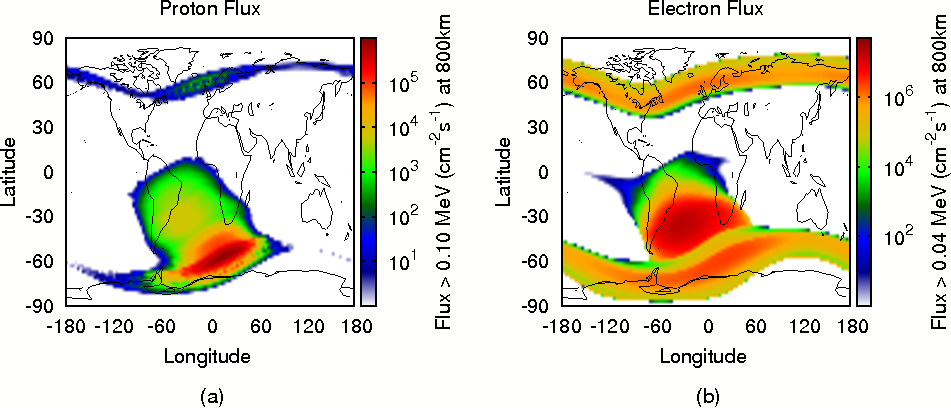
\includegraphics[width=0.6\paperwidth]{img/03/polar_SAA.png}
        \caption{Radiation pattern on LEO. Source: \cite{ESA_radiation}}
         \label{Polar_SAA}
    \end{figure}

    \bigskip \textbf{Solar flares}

    During solar flares large fluxes of protons are produced, and some of these reach Earth. Earth's magnetic field provides some shielding from them, but they may become trapped inside, easily reaching polar regions and South Atlantic Anomaly. Solar flares are unpredictable, and represent a threat to spacecraft operations.

    \bigskip \textbf{Cosmic rays}

    Cosmic rays originate from outside the solar system. They are very high energy particles, making effective shielding very difficult. Flux of this kind of particle is low, therefore they mostly contribute to single-event processes.

\section{Radiation effects on electronic devices}
    There are two basic effects of radiation on silicon components:
    \begin{itemize}
         \item ionizing effect
        \item displacement damage
    \end{itemize}

    These two effect are responsible for changing the parameters of semiconductor devices, which after some time can lead to failure of the device. The main source of this radiation are gamma (ionization) and neutron particles (displacement).

    In space electronics during analysis and design two major problems are considered - Single Event Effects (SEE) and Total Ionizing Dose (TID). Every silicon and silica device is susceptible to both of those - and both have to be considered during product design, development and testing.

    \subsection{Single Event Effects}
        Single Event Effects are connected with the generation of electron-hole pairs in semiconductor material when exposed to ionizing radiation. The number of pairs generated is proportional to the energy deposited. For semiconductor devices, the parameter $LET_{th}$ (Linear Energy Transfer Threshold) is defined, being a measure of how susceptible the device is. For particles with Linear Energy Transfer (LET - normalized particle energy per mass of the absorbing material), below this threshold no effect will be observed.

        Single Event Effects are divided into two groups - non-destructive (fully recoverable, possibly after power cycle) and destructive (permanent damage) effects. These are described below, defined as in \cite{ECSS_Q_ST_60_15C}.

        \bigskip\textbf{Non-destructive effects}
        \begin{itemize}
            \item \textbf{Single Event Upset} - especially vulnerable are memory-based devices (like microprocessors, memories, Field Programmable Gate Array - FPGA etc). This phenomenon may alter the state of cells in memory - causing memory corruption. This can lead to complete device failure if not corrected.

            \item \textbf{Single Event Functional Interrupt} - subset of SEU - this effect causes the system to latch in a non-recoverable state (e.g. by switching to wrong state in state machine). The only option is to reset the circuit to back to a known state.

            \item \textbf{Single Event Transient} - are formed as spurious voltage/current pulses generated by the charge induced by striking particles. This can cause a variety of problems - from the disturbing of analog electronics to the anomalous switching of digital circuits. This effect strongly depends on the size of the feature in silica.
        \end{itemize}

        \bigskip\textbf{Destructive effects}
        \begin{itemize}
            \item \textbf{Single Event Latch-up} - particle striking can cause the activation of a parasitic thyristor in the CMOS structure. This will lead to effectively shorting the voltage supply to ground, causing overheat and damage to the device.

            \item \textbf{Single Event Gate Rupture} - high energy particles coming through the thin gate (especially in MOS transistors) can cause generation of electron-hole pairs in gate and substrate - causing a high electric field across the gate. When this effect is strong enough it can cause permanent damage to the transistor.

            \item \textbf{Single Event Burnout} - an ion that traverses the transistor structure (through the source) can induce a current flow that turns on the parasitic npn transistor. This leads to effective short circuiting and damage to the device.
        \end{itemize}

        \bigskip\textbf{Mitigation techniques}

        Below recommended mitigation techniques for SEE are listed:
        \begin{itemize}
            \item SEU - redundancy, memory scrubbing,
            \item SEFI - watchdog, proper reset sequence,
            \item SET - use lower-integration scale devices, implement protection resistors etc.
            \item SEL - implement overcurrent circuits (like Latch-up Current Limiters),
            \item SEGR, SEB - use higher $LET_{th}$ devices
        \end{itemize}

    \subsection{Total Ionizing Dose}
        TID is defined as the total energy absorbed during exposure. This can be caused by any kind of radiation, behaving differently in every semiconductor device. In general, TID successively degrades electronic device parameters over time, causing them to stop functioning when critical irradiation is reached. The effect in p-MOSFET transistors is described in section \ref{Radiation_effects_on_MOS_transistors}.

\section{Need for TID radiation dosimetry}
    During spacecraft missions, accumulated radiation levels should be monitored in order not to exceed certain guaranteed values for components. For example, near the end of its lifetime, a spacecraft can be commanded to deorbit into the atmosphere or move to graveyard orbit - before failure can occur, causing loss of control of the spacecraft, like for example in Telstar-1.
    Absorbed dose simulation is a good method of its estimation, but, because radiation flux varies (due to cosmic events like solar flares), errors can accumulate during a satellite's lifetime. Flying by the South Atlantic Anomaly or Van Allen belts can cause inaccuracies in radiation estimations, so nearly all spacecraft implement sensors which constantly monitor the radiation levels absorbed by their electronics.

\section{On-line TID radiation dosimetry}
    A number of possible dosimetry methods were considered:
    \begin{itemize}
        \item PIN diode - forward voltage shift during irradiation \cite{PIN_dosimetry},
        \item memory dosimetry - single events cause bit flips in memory - accumulated number of errors reflects absorbed dose \cite{RadFET_PhD},
        \item FGMOSFET - change in differential channel current - indicative of radiation dose \cite{FGMOSFET_patent},
        \item RadFET - shift of threshold voltage of p-MOS transistor indicates irradiation \cite{RadFET_PhD}.
    \end{itemize}
    Detailed description of those dosimetry methods can be found in \cite{RadFET_PhD}.

    For this sensor, it was decided to use RadFET as a sensing element. These kinds of sensor have already flown on many satellites and are used in medical and industrial dosimetry.

    The most important advantages of RadFET dosimetry:
    \begin{itemize}
        \item sensor can be completely shut down during irradiation (no power consumption and reduced reliability issues),
        \item integrated measurement (especially important for small dose rates),
        \item on-line, non-destructive readout,
        \item small size,
    \end{itemize}
    And the most crucial drawbacks:
    \begin{itemize}
        \item low sensitivity - requires sophisticated measurement setup,
        \item required temperature compensation.
    \end{itemize}


\section{RadFET Theory}
    The basic idea of RadFET, using metal-oxide semiconductor field-effect transistors (MOSFET), is to measure the threshold voltage shift, $\Delta V_{TH}$ and convert it into an absorbed dose.

    \subsection{Radiation effects on MOS transistors}
    \label{Radiation_effects_on_MOS_transistors}
        Irradiation of MOSFET transistor results in threshold voltage shift. This is caused by trapping of holes (generated during particle strike) and creation of interface states on gate/bulk boundary. Those effects are shown in the figure \ref{MOS_irradiation} \cite{pMOS_dosimeters_radfets}.

        \begin{figure}[H]
            \centering
            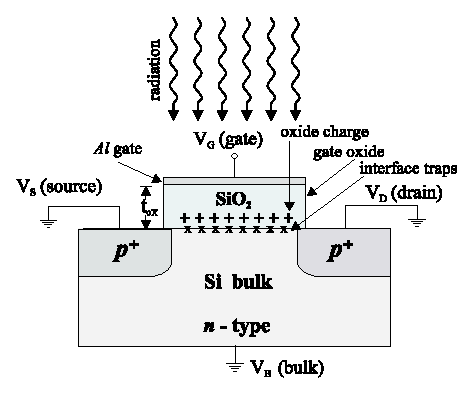
\includegraphics[width=0.4\paperwidth]{img/03/MOS_irradiation_schematic.eps}
            \caption{pMOS irradiation schematic. Source: \cite{pMOS_dosimeters_radfets}}
            \label{MOS_irradiation}
        \end{figure}

        Threshold voltage will shift according to the following equation \cite{pMOS_dosimeters_radfets}:

        $$\Delta V_{TH} = A \cdot D^n$$

        Where:

        \begin{tabular}{lcl}
            $\Delta V_{TH}$ & - & threshold voltage shift \\
            $A$ & - & constant \\
            $D$ & - & absorbed dose \\
            $n$ & - & degree of linearity (ideally $n = 1$) \\
        \end{tabular}
        \bigskip



    \subsection{Threshold voltage measurement}
        The simplest method to measure threshold voltage shift is to use diode configuration of MOS transistor, current source and measure voltage across, as shown in the figure \ref{MOS_measurement_setup}.

        \begin{figure}[H]
            \centering
            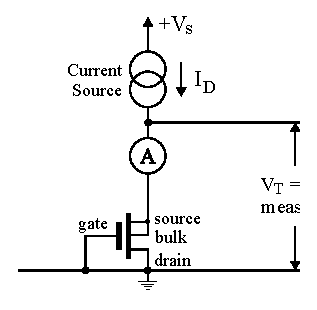
\includegraphics[width=0.3\paperwidth]{img/03/Vth-measurement-setup.eps}
            \caption{Measurement setup. Source: \cite{pMOS_dosimeters_radfets}}
            \label{MOS_measurement_setup}
        \end{figure}

    \subsection{Temperature dependencies}
        Threshold voltage of transistor strongly depends on die temperature \cite{managing_temperature_effects_in_nanoscale_adaptive_systems}.

        This dependency is usually described to be linear:

        $$\Delta V_{TH} = A \cdot \Delta T$$

        Where:

        \begin{tabular}{lcl}
            $\Delta V_{TH}$ & - & threshold voltage shift \\
            $A$ & - & constant \\
            $\Delta T$ & - & temperature change \\
        \end{tabular}
        \bigskip

        Constant coefficient depends on particular MOSFET, technology and (very weakly) irradiation. Usually this coefficient is in the range $-0.1$ to \SI{-1}{\milli\volt/\kelvin}.
